\documentclass{article}
\usepackage{amssymb}
\usepackage{changepage}
\usepackage{amsmath}
\usepackage{gensymb}
\usepackage{cancel}
\usepackage{tkz-euclide}
\usepackage{graphicx}
\title{Momentum and Energy Summary}
\author{Tristan Simpson}
\begin{document}
\maketitle

\section{Equations}
\begin{adjustwidth}{1cm}{0pt}
    \subsection{Energy without a spring}
    \begin{flushleft}
        The value of $E_{k}$ is dependant on whether the object begins with any motion. The variable $E_{g}$ is dependant on whether the object begins with / ends with a specific height.\newline\newline
        $E_{tot} = E_{tot}\prime$ \\
        \vspace*{10pt}
        $E_{k} + E_{g} = E_{k}\prime + E_{g}\prime$ \\
        \vspace*{10pt}
        $(\frac{1}{2}mv^2) + (mgh) = (\frac{1}{2}mv^2)\prime + (mgh)\prime$
    \end{flushleft}
    \subsection{Energy with a spring}
    \begin{flushleft}
        If a force/object pushing on the spring, then the variable $E_{e}$ has a value. Else, set it's value to zero. With this being, if an object is being dropped onto a spring, only $E_{e}\prime$ has a value.\newline\newline
        $E_{tot} = E_{tot}\prime$ \\
        \vspace*{10pt}
        $E_{k} + E_{g} + E_{e} = E_{k}\prime + E_{g}\prime + E_{e}\prime$ \\
        \vspace*{10pt}
        $(\frac{1}{2}mv^2) + (mgh) + (\frac{1}{2}kx^2) = (\frac{1}{2}mv^2)\prime + (mgh)\prime + (\frac{1}{2}kx^2)\prime$
    \end{flushleft}
    \subsection{Momentum (1)}
    \begin{flushleft}
        The two objects do \textbf{\textit{not}} move together after colliding. Instead, they seperate from eachother, both moving in different paths.\newline\newline
        $P_{tot} = P_{tot}\prime$ \\
        \vspace*{10pt}
        $P_{a} + P_{b} = P_{a}\prime + P_{b}\prime$ \\
        \vspace*{10pt}
        $(m_{a})(v_{a}) + (m_{b})(v_{b}) = (m_{a})(v_{a})\prime + (m_{b})(v_{b})\prime$
    \end{flushleft}
    \vspace*{0.03cm}
    \subsection{Momentum (2)}
    \begin{flushleft}
        The two objects move together after colliding. Instead of seperating from eachother, both objects have conjoined, each moving in the same path.\newline\newline
        $P_{tot} = P_{tot}\prime$ \\
        \vspace*{10pt}
        $P_{a} + P_{b} = P_{ab}$ \\
        \vspace*{10pt}
        $(m_{a})(v_{a}) + (m_{b})(v_{b}) = (m_{a + b})(v_{a\times b})$
    \end{flushleft}
\end{adjustwidth}

\section{Units}
\begin{adjustwidth}{1cm}{0pt}
    \begin{minipage}{0.33\textwidth}
        \begin{itemize}
            \item $F_{s} = N$
            \item $k = \frac{N_{ewtons}}{m_{eter}}$
            \item $x = m_{eters}$
            \item $P_{tot} = \frac{kgm}{s}$
        \end{itemize}
    \end{minipage}
    \begin{minipage}{0.33\textwidth}
        \begin{itemize}
            \item $E_{e} = J$
            \item $W = J$
            \item $\Delta E = J$
            \item $E_{tot} = J$
        \end{itemize}
    \end{minipage}
\end{adjustwidth}

\vspace*{0.5cm}
\section{Collisions}
\begin{adjustwidth}{1cm}{0pt}
    \subsection*{Elastic vs. In-Elastic}
    \begin{adjustwidth}{0.5cm}{0pt}
        In an ELASTIC collision, the kinetic energy of the SYSTEM is equal before and after the collision.  In an INELASTIC collision, the kinetic energy of the SYSTEM is NOT equal between the before and after of the collision.\newline\newline
        An elastic collision occurs when two objects collide and are physically the same after the collision as they were before the collision. An inelastic collision occurs when the physical shape of the objects involved has been altered and is different after compared to before the collision.
    \end{adjustwidth}
    \subsection*{Calculation Steps}
    \begin{flushleft}
        If you get stuck on a problem, try to use $P_{tot} = P_{tot}\prime$ and/or $E_{tot} = E_{tot}\prime$ to solve for what you need.
    \end{flushleft}
    \vspace*{5pt}
    \begin{adjustwidth}{0.5cm}{0pt}
        \begin{enumerate}
            \item Diagram
            \item Givens
            \item What are you looking for?
            \item $P_{tot} = P_{tot}\prime$ or $E_{tot} = E_{tot}\prime$
        \end{enumerate}
    \end{adjustwidth}
\end{adjustwidth}

\section{Energy and Springs}
\begin{adjustwidth}{1cm}{0pt}
    \subsection*{Calculation Steps (No 5 Steps)}
    \begin{flushleft}
        Recall Hooke's Law (The extension or compression of a spring). $E_{e}$ is Elastic Potential Energy - The stored energy in a spring from it's compression or extension.
    \end{flushleft}
    \vspace*{5pt}
    \begin{adjustwidth}{0.5cm}{0pt}
        \begin{enumerate}
            \item $F_{s} = kx$ or $k = \frac{F_{s}}{x}$
            \item $E_{k} + E_{g} + E_{e} = E_{k}\prime + E_{g}\prime + E_{e}\prime$
        \end{enumerate}
    \end{adjustwidth}
\end{adjustwidth}

\section{Impulses}
\begin{adjustwidth}{1cm}{0pt}
    \subsection*{Equations}
    \begin{flushleft}
        Impulses do not require components. Rearrange the equations below to solve for what you need.
    \end{flushleft}
    \vspace*{7pt}
    \noindent
    \begin{minipage}{0.33\textwidth}
        \begin{itemize}
            \item $\Delta P = m\Delta v$
            \item $\Delta P = ma\Delta t$
            \item $\Delta P = F_{net}\Delta t$
        \end{itemize}
    \end{minipage}
    \begin{minipage}{0.33\textwidth}
        \begin{itemize}
            \item $a = \frac{\Delta v}{\Delta t}$
            \item $\Delta v = a \Delta t$
            \item $F_{net} = ma$
            \item $\Delta v = (v_{2} - v_{1})$
        \end{itemize}
    \end{minipage}
    \subsection*{Calculation Steps}
    \begin{flushleft}
        Impulses are about the push back of an opposing force.
    \end{flushleft}
    \vspace*{5pt}
    \begin{adjustwidth}{0.5cm}{0pt}
        \begin{enumerate}
            \item Diagram
            \item Givens
            \item What are you looking for?
            \item Use the equations above to solve for what you need.
        \end{enumerate}
    \end{adjustwidth}
\end{adjustwidth}

\section{2D Momentum}
\begin{adjustwidth}{1cm}{0pt}
    \subsection*{Calculation Steps}
    \begin{flushleft}
        Similar to collisions except it includes both $x$ and $y$ components.
    \end{flushleft}
    \vspace*{5pt}
    \begin{adjustwidth}{0.5cm}{0pt}
        \begin{enumerate}
            \item Diagram
            \item Givens
            \item What are you looking for?
            \item Components
            \item $P_{tot_{x}} = P_{tot_{x}}\prime$ and $P_{tot_{y}} = P_{tot_{y}}\prime$
            \item $c^2 = a^2 + b^2$
        \end{enumerate}
    \end{adjustwidth}
\end{adjustwidth}

\section{Example Equations}
\begin{adjustwidth}{1cm}{0pt}
    \subsection*{7.1\hspace*{0.5cm}2D Momentum - Question}
    \begin{flushleft}
        A billiard ball with a mass of 0.155kg is rolling directly
        away from you at 3.5 $\frac{m}{s}$. It collides with a stationary golf ball with
        a mass of 0.05kg. The billiard ball rolls off at an angle of $15\degree$ clockwise
        from it's original direction with a velocity of $3.1\frac{m}{s}$. What is the after
        velocity of the golf ball?
    \end{flushleft}
    \subsection*{7.1\hspace*{0.5cm}2D Momentum - Graph and Givens}
    \begin{minipage}{0.5\textwidth}
        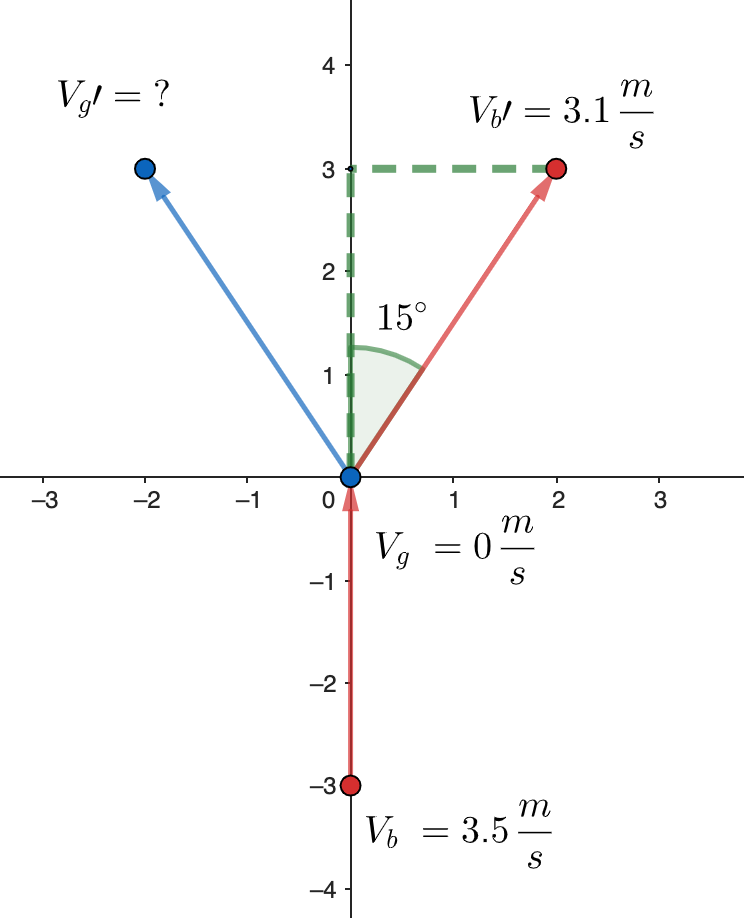
\includegraphics[scale=0.33]{./images/2d_momentum_graph}
    \end{minipage}
    \begin{minipage}{0.5\textwidth}
        \begin{itemize}
            \item $m_{b} = 0.155kg$
            \item $m_{g} = 0.052kg$
            \item $V_{b} = 3.5\frac{m}{s}$
            \item $V_{g} = 0\frac{m}{s}$
            \item $V_{b}\prime = 3.1\frac{m}{s}$ $[15\degree clockwise]$
            \item $V_{g}\prime = ?$
        \end{itemize}
    \end{minipage}
    \subsection*{7.1\hspace*{0.5cm}2D Momentum - Solve}
    This solve requires both $x$ and $y$ components. Since $v_{b}$ only has a $y$ direction, $v_{b_{x}}$ is zero. Also, since $v_{g}$ isn't moving, both $v_{g_{x}}$ and $v_{g_{y}}$ are zero.\newline\newline
    \textbf{1.} $P_{tot_{x}} = P_{tot_{x}}\prime$ \\
    \begin{adjustwidth}{0.6cm}{0pt}
        $(m_{g})(\cancel{v}_{g_{x}}^0) + (m_{b})(\cancel{v}_{b_{x}}^0) = (m_{g})(v_{g_{x}}\prime) + (m_{b})(v_{b_{x}}\prime)$ \\\\
        $\therefore v_{g_{x}}\prime = -\left(\frac{(m_{b})(v_{b_{x}}\prime)}{m_{g}}\right) = -\left(\frac{(0.155)(3.1\sin15\degree)}{(0.052)}\right)$
    \end{adjustwidth}\vspace*{15pt}
    \textbf{2.} $P_{tot_{y}} = P_{tot_{y}}\prime$ \\
    \begin{adjustwidth}{0.6cm}{0pt}
        $(m_{g})(\cancel{v}_{g_{y}}^0) + (m_{b})(v_{b_{y}}) = (m_{g})(v_{g_{y}}\prime) + (m_{b})(v_{b_{y}}\prime)$ \\\\
        $\therefore v_{g_{y}}\prime = \left(\frac{(m_{b})(v_{b_{y}}) - (m_{b})(v_{b_{y}}\prime)}{m_{g}}\right) = \left(\frac{(0.155)(3.5) - (0.155)(3.1\cos15\degree)}{0.052}\right)$
    \end{adjustwidth}\vspace*{15pt}
    \noindent\textbf{3.} Use $c^2 = a^2 + b^2$ \\
    \begin{adjustwidth}{0.6cm}{0pt}
        $\therefore v_{g}\prime = \sqrt[]{{(v_{g_{x}}\prime)}^2 + {(v_{g_{y}}\prime)}^2} = \sqrt[]{{(-2.391)}^2 + {(1.507)}^2} \approx 2.766 \frac{m}{s} $
    \end{adjustwidth}

    \subsection*{7.2\hspace*{0.5cm}Inelastic Momentum - Question}
    A child with a mass of 22 kg runs at a horizontal velocity of 4.2 m/s [forward] and jumps onto a stationary rope swing of mass 2.6 kg. The child "sticks" on the rope swing and swings forward.
    \subsection*{7.2\hspace*{0.5cm}Inelastic Momentum - Givens}
    Determine the horizontal velocity of the child plus the swing just after impact then determine the height that the child and swing rise.\newline\newline
    \begin{minipage}{0.5\textwidth}
        
\includegraphics[scale=0.33]{./images/child_rope}
    \end{minipage}
    \begin{minipage}{0.5\textwidth}
        \begin{itemize}
            \item $m_{c} = 22kg$
            \item $m_{r} = 2.6kg$
            \item $v_{c} = 4.2\frac{m}{s}$
            \item $v_{r} = 0\frac{m}{s}$
            \item $v_{cr} = ?$
            \item $h_{cr} = ?$
        \end{itemize}
    \end{minipage}
    \subsection*{7.2\hspace*{0.5cm}Inelastic Momentum - Solve}
    Whilst using the formula $E_{tot} = E_{tot}\prime$ the variable $E_{k}\prime$ is set to zero because when the child reaches his max height, $v = 0$ thus $E_{k} = 0$\newline\newline
    \textbf{1.} $P_{tot_{x}} = P_{tot_{x}}\prime$ \\
    \begin{adjustwidth}{0.6cm}{0pt}
        $(m_{c})({v}_{c}) + (m_{r})(\cancel{v}_{r}^0) = (m_{c + r})(v_{cr})$ \\\\
        $\therefore v_{cr} = \left(\frac{(m_{c})(v_{c})}{(m_{c + r})}\right) = \left(\frac{(22)(4.2)}{(22 + 2.6)}\right) \approx 3.7\frac{m}{s}$
    \end{adjustwidth}\vspace*{15pt}
    \textbf{2.} $E_{tot_{y}} = E_{tot_{y}}\prime$ \\
    \begin{adjustwidth}{0.6cm}{0pt}
        $(m_{c}g\cancelto{0}{h}) + (\frac{1}{2}m_{c}v_{c}^2) = (m_{c + r}gh)\prime + \cancelto{0}{(\frac{1}{2}m_{c}v_{c}^2)\prime}$ \\\\
        $\therefore h = \left(\frac{(m_{c}v_{c}^2)}{2(m_{c+r}g)}\right) = \left(\frac{(22){(4.2)}^2}{2(22 + 2.6)(9.81)}\right) \approx 1.6m$
    \end{adjustwidth}\vspace*{15pt}

    \subsection*{7.3\hspace*{0.5cm}Elastic Momentum - Question}
    Jeremey and Griffin are stupid and throw two live hand grenades at each other to see what happens. Hand grenade A is travelling at a velocity of 3.0m/s with a mass of 1.2kg. Hand grenade B is travelling at a velocity of 2.7m/s with a mass of 1.3kg. What is the velocity of the two objects after they collide?
    \subsection*{7.3\hspace*{0.5cm}Elastic Momentum - Graph and Givens}
    Determine the velocity of Hand Grenade A and Hand Grenade B post-collision.\newline\newline
    \begin{minipage}{0.5\textwidth}
        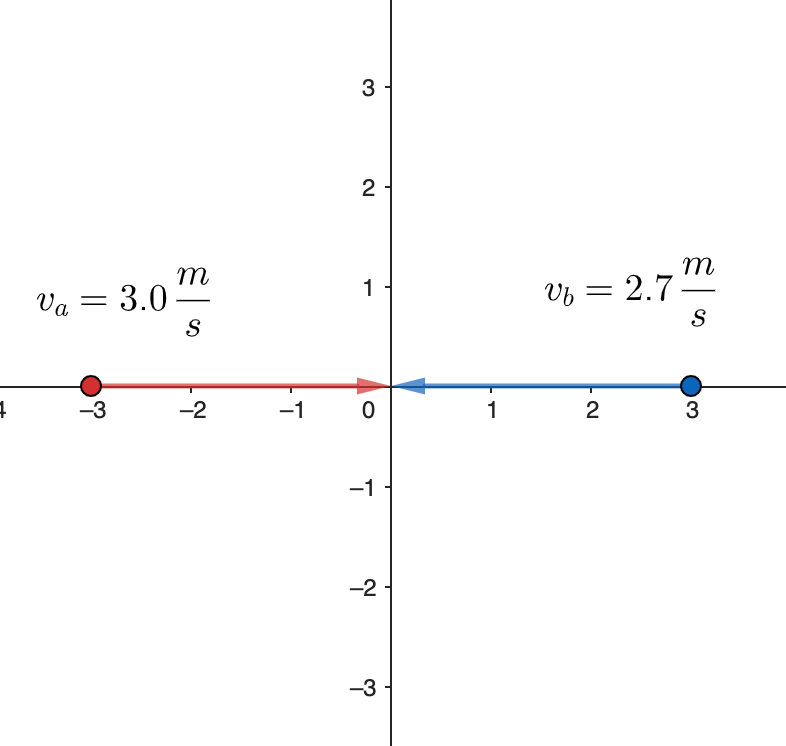
\includegraphics[scale=0.33]{./images/elastic_collision}
    \end{minipage}
    \begin{minipage}{0.5\textwidth}
        \begin{itemize}
            \item $m_{a} = 1.2g$
            \item $m_{b} = 1.3kg$
            \item $v_{a} = 3.0\frac{m}{s}$
            \item $v_{b} = 2.7\frac{m}{s}$
            \item $v_{a}\prime = ?$
            \item $v_{b}\prime = ?$
        \end{itemize}
    \end{minipage}
    \subsection*{7.3\hspace*{0.5cm}Elastic Momentum - Solve}
    Because of the law of conservation of momentum, this equation is Elastic. The velocity of the objects will be same as they were before the collision.\newline\newline
    \textbf{1.} $P_{tot} = P_{tot}\prime$ \\
    \begin{adjustwidth}{0.6cm}{0pt}
        $(\cancel{m_{a}})({v}_{a}) + (\cancel{m_{b}})({v}_{b}) = (\cancel{m_{a}})({v}_{a})\prime + (\cancel{m_{b}})({v}_{b})\prime$ \\\\
        $({v}_{a}) + ({v}_{b}) = ({v}_{a})\prime + ({v}_{b})\prime$ \\\\
        $\therefore v_{a}\prime = v_{a} = 3.0\frac{m}{s}$ \\\\
        $\therefore v_{b}\prime = v_{b} = 2.7\frac{m}{s}$
    \end{adjustwidth}\vspace*{15pt}
    \textbf{2.} Proof of Elastic with $E_{tot} = E_{tot}\prime$ \\
    \begin{adjustwidth}{0.6cm}{0pt}
        $\frac{1}{2}mv_{a} + \frac{1}{2}mv_{b} = \frac{1}{2}mv_{a}\prime + \frac{1}{2}mv_{b}\prime$ \\\\
        $\frac{1}{2}(1.2)(3.0) + \frac{1}{2}(1.3)(2.7) = \frac{1}{2}(1.2)(3.0) + \frac{1}{2}(1.3)(2.7)$ \\\\
        $\therefore$ Elastic $3.055 = 3.055$
    \end{adjustwidth}\vspace*{15pt}

    \subsection*{7.4\hspace*{0.5cm}Energy with Spring - Question}
    A low friction cart with a mass of 0.25kg travels along a horizontal track and collides
    head on with a spring that has a spring constant of $155\frac{N}{m}$.
    If the Spring was compressed by 6.0cm, how fast was the cart initially travelling?
    \subsection*{7.4\hspace*{0.5cm}Energy with Spring - Graph and Givens}
    \begin{minipage}{0.5\textwidth}
        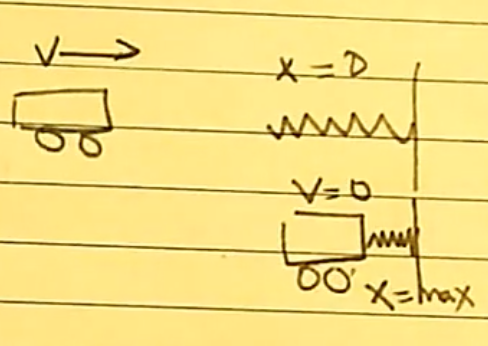
\includegraphics[scale=0.33]{./images/springs.png}
    \end{minipage}
    \begin{minipage}{0.5\textwidth}
        \begin{itemize}
            \item $x = 6.0cm$
            \item $k = 155\frac{N}{m}$
            \item $m_{c} = 0.25kg$
            \item $v_{c} = ?$
        \end{itemize}
    \end{minipage}
    \subsection*{7.4\hspace*{0.5cm}Energy with Spring - Solve}
    Because the cart is not initially colliding with the spring, $E_{e}$ is zero. Because the cart's velocity post-collision is zero, $E_{k}$ is also zero. Because the cart and the spring are at the same height both before and after the collision, both $E_{g}$ and $E_{g}\prime$ are set to zero.\newline\newline
    \textbf{1.} $E_{tot} = E_{tot}\prime$ \\
    \begin{adjustwidth}{0.6cm}{0pt}
        $E_{k} + \cancelto{0}{E_{g}} + \cancelto{0}{E_{e}} = \cancelto{0}{E_{k}\prime} + \cancelto{0}{E_{g}\prime} + E_{e}\prime$ \\\\
        $E_{k} = E_{e}\prime$ \\\\
        $\frac{1}{2}m_{c}v_{c}^2 = \frac{1}{2}kx^2$ \\\\
        $\therefore v_{c} = \sqrt[]{\frac{kx^2}{m_{c}}} = \sqrt[]{\frac{(155){(6.0)}^2}{(0.25)}} \approx 149\frac{m}{s}$
    \end{adjustwidth}\vspace*{15pt}
    \textbf{2.} $h_{c} = 9.2m$ \\
    \begin{adjustwidth}{0.6cm}{0pt}
        $E_{k} + E_{g} + \cancelto{0}{E_{e}} = \cancelto{0}{E_{k}\prime} + \cancelto{0}{E_{g}\prime} + E_{e}\prime$ \\\\
        $E_{k} + E_{g} = E_{e}\prime$ \\\\
        $\frac{1}{2}m_{c}v_{c}^2 + m_{c}gh = \frac{1}{2}kx^2$ \\\\
        $\therefore v_{c} = \sqrt[]{\frac{(kx^2) - (m_{c}gh)}{m_{c}}} = \sqrt[]{\frac{(155){(6.0)}^2 - (0.25)(9.81)(9.2)}{(0.25)}} \approx 149\frac{m}{s}$
    \end{adjustwidth}\vspace*{15pt}


    \subsection*{7.5\hspace*{0.5cm}Energy + Momentum - Question (Boulder)}
    A 55.6 kg boulder sat on the side of a mountain beside a lake. The boulder was 14.6 m
    above the surface of the lake. One winter
    night, the boulder rolled down the mountain,
    directly into a 204 kg ice-fishing shack that
    was sitting on the frozen lake. What was the
    velocity of the boulder and shack at the
    instant that they began to slide across the
    ice?
    \subsection*{7.5\hspace*{0.5cm}Energy + Momentum - Graph and Givens}
    \begin{minipage}{0.5\textwidth}
        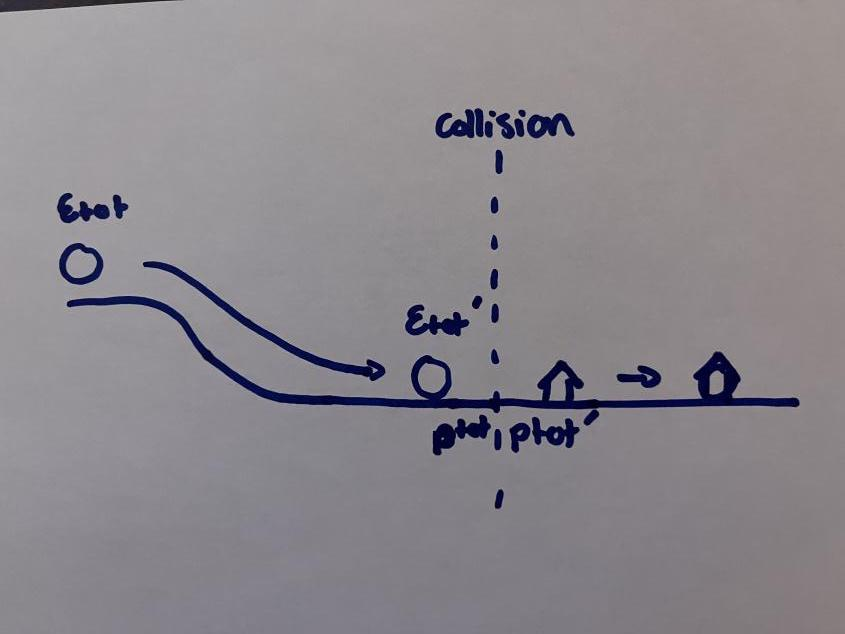
\includegraphics[scale=0.2]{./images/boulder.png}
    \end{minipage}
    \begin{minipage}{0.5\textwidth}
        \begin{itemize}
            \item $m_{b} = 55.6kg$
            \item $m_{s} = 204kg$
            \item $h_{b} = 14.6m$
            \item $h_{s} = 0m$
            \item $v_{bs} = ?$
        \end{itemize}
    \end{minipage}
    \subsection*{7.5\hspace*{0.5cm}Energy + Momentum - Solve}
    Because the cart is not initially colliding with the spring, $E_{e}$ is zero. Because the cart's velocity post-collision is zero, $E_{k}$ is also zero. Because the cart and the spring are at the same height both before and after the collision, both $E_{g}$ and $E_{g}\prime$ are set to zero.\newline\newline
    \textbf{1.} $E_{tot} = E_{tot}\prime$ \\
    \begin{adjustwidth}{0.6cm}{0pt}
        $\cancelto{0}{E_{k}} + E_{g} = E_{k}\prime + \cancelto{0}{E_{g}\prime}$ \\\\
        $(m_{b})(g)(h_{b}) = \frac{1}{2}m_{b}v_{b}^2$ \\\\
        $\therefore v_{b} = \sqrt[]{\frac{(2)(m_{b})(g)(h_{b})}{m_{b}}} = \sqrt[]{\frac{(2)(55.6)(9.81)(14.6)}{(55.6)}} \approx 16.9\frac{m}{s}$
    \end{adjustwidth}\vspace*{15pt}
    \textbf{2.} $P_{tot} = P_{tot}\prime$ \\
    \begin{adjustwidth}{0.6cm}{0pt}
        $m_{b}v_{b} + m_{s}\cancelto{0}{v_{s}} = m_{b + s}v_{bs}$ \\\\
        $\therefore v_{bs} = \frac{m_{b}v_{b}}{m_{b + s}} = \frac{(55.6)(16.9)}{(55.6 + 204)} \approx 3.61\frac{m}{s}$
    \end{adjustwidth}\vspace*{15pt}


    \subsection*{7.6\hspace*{0.5cm}Impulses - Question}
    Jen has a mass of 50kg and is in a car going $35\frac{m}{s}$ when she gets in an accident. The airbags deploy and bring her body to a stop in 0.500s. What is the force applied to her body?
    \subsection*{7.6\hspace*{0.5cm}Impulses - Givens}
    \begin{minipage}{0.5\textwidth}
        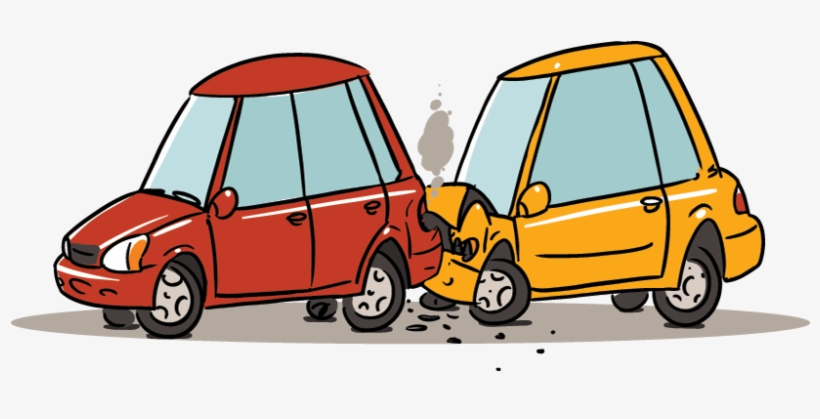
\includegraphics[scale=0.2]{./images/car_crash.png}
    \end{minipage}
    \begin{minipage}{0.5\textwidth}
        \begin{itemize}
            \item $v_{1} = 35\frac{m}{s}$
            \item $v_{2} = 0\frac{m}{s}$
            \item $\Delta t = 0.500s$
            \item $m_{J} = 50kg$
        \end{itemize}
    \end{minipage}
    \subsection*{7.6\hspace*{0.5cm}Impulses - Solve}
    We can solve this problem using the equations provided in the Impulses section of this big book.\newline\newline
    \textbf{1.} $\Delta P = F_{net}\Delta t$ \\
    \begin{adjustwidth}{0.6cm}{0pt}
        $F_{net} = \frac{\Delta P}{\Delta t} = \frac{m\Delta v}{\Delta t} = \frac{m(v_{2} - v_{1})}{\Delta t}$ \\\\
        $\therefore F_{net} = \frac{50(0 - 35)}{0.500} \approx -3500N$
    \end{adjustwidth}\vspace*{15pt}
    \textbf{2.} $t = 0.100s$ \\
    \begin{adjustwidth}{0.6cm}{0pt}
        $F_{net} = \frac{\Delta P}{\Delta t} = \frac{m\Delta v}{\Delta t} = \frac{m(v_{2} - v_{1})}{\Delta t}$ \\\\
        $\therefore F_{net} = \frac{50(0 - 35)}{0.100} \approx -17500N$
    \end{adjustwidth}\vspace*{15pt}
    \subsection*{7.6\hspace*{0.5cm}Impulses - Note}
    Therefore if the time is lower, the less force the collision has on the person. This is why airbags are so important. Airbags reduce the time within the equation.

\end{adjustwidth}
\end{document}